\documentclass[12pt,a4paper,oneside]{article}

% ============================================
% PACKAGES
% ============================================
\usepackage[margin=2.5cm]{geometry}
\usepackage{xcolor}
\usepackage{amsmath,amssymb}
\usepackage{listings}
\usepackage{booktabs}
\usepackage{longtable}
\usepackage{array}
\usepackage{tabularx}
\usepackage{hyperref}
\usepackage{graphicx}
\usepackage{ragged2e}
\usepackage{microtype}
\usepackage{parskip}
\usepackage{enumitem}
\usepackage{fancyhdr}
\usepackage{titlesec}
\usepackage{float}
\usepackage{subcaption}
\newcolumntype{Y}{>{\raggedright\arraybackslash}X}

% ============================================
% IMAGE PATHS + ROBUST FIGURE SLOTS
% ============================================
% Drop diagram renders in docs/ (ER_MODEL.png, WF_DIAGRAM.png, architecture.png)
% Drop screenshots / photos in docs/team/images/  (create the folder)
\graphicspath{{./}{../}{./images/}{../images/}}

% \figslot[width]{filename}{caption}{label}
% Renders the image if it exists; otherwise a labelled placeholder box so the
% document ALWAYS compiles. Replace the box by dropping the named file in place.
\newcommand{\figslot}[4][0.92]{%
  \begin{figure}[H]
    \centering
    \IfFileExists{#2}{%
      \includegraphics[width=#1\textwidth]{#2}%
    }{%
      \fbox{\parbox[c][4.5cm][c]{0.88\textwidth}{\centering\itshape
        [\,Paste image here\,]\\[4pt]
        expected file: \texttt{\detokenize{#2}}}}%
    }
    \caption{#3}\label{#4}
  \end{figure}
}

% ============================================
% COLOR DEFINITIONS
% ============================================
\definecolor{linkblue}{RGB}{41,121,255}
\definecolor{codegray}{RGB}{240,240,240}
\definecolor{codegreen}{RGB}{0,128,0}
\definecolor{codegray}{RGB}{128,128,128}

% ============================================
% LISTINGS SETUP
% ============================================
\lstset{
    backgroundcolor=\color{codegray},
    basicstyle=\ttfamily\footnotesize,
    breaklines=true,
    captionpos=b,
    commentstyle=\color{codegreen},
    frame=single,
    keepspaces=true,
    keywordstyle=\color{blue},
    numbers=left,
    numbersep=5pt,
    numberstyle=\tiny\color{codegray},
    showspaces=false,
    showstringspaces=false,
    showtabs=false,
    tabsize=2
}

% Custom listings languages (TypeScript / JSON / Dockerfile are not built in)
\lstdefinelanguage{TypeScript}{
  morekeywords={async,await,const,let,var,return,for,while,if,else,import,from,export,
    class,new,function,of,in,this,interface,type,enum,boolean,number,string,Promise,
    void,private,public,readonly,extends,implements,true,false,null,undefined},
  sensitive=true,
  morecomment=[l]{//},
  morecomment=[s]{/*}{*/},
  morestring=[b]',
  morestring=[b]",
  morestring=[b]`,
}
\lstdefinelanguage{JSON}{
  morestring=[b]",
  morecomment=[l]{//},
}
\lstdefinelanguage{Dockerfile}{
  morekeywords={FROM,RUN,CMD,ENV,COPY,ADD,WORKDIR,EXPOSE,ENTRYPOINT,VOLUME,version,
    services,build,ports,environment,depends_on,image},
  sensitive=false,
  morecomment=[l]{\#},
}

% ============================================
% HYPERREF SETUP
% ============================================
\hypersetup{
    colorlinks=true,
    linkcolor=linkblue,
    urlcolor=linkblue,
    citecolor=linkblue,
    pdfauthor={Ismail (ismoiljon1101)},
    pdftitle={Fishlinic -- End-to-End Software + Hardware Documentation},
    pdfsubject={Sejong University Capstone Design Project 2026}
}

% ============================================
% HEADER/FOOTER
% ============================================
\pagestyle{fancy}
\fancyhf{}
\fancyhead[L]{Fishlinic -- Sejong University Capstone}
\fancyhead[R]{\thepage}
\fancyfoot[C]{CTO-Level Technical Documentation -- v3.0}

% ============================================
% TITLE PAGE
% ============================================
\title{
    \vspace{2cm}
    \Huge\textbf{Fishlinic}\\
    \Large\textbf{End-to-End Software + Hardware Documentation}\\
    \vspace{1cm}
    \large\textit{CTO-Level Technical Documentation}\\
    \large\textit{Sejong University Capstone Design Project 2026}
    \vspace{2cm}
}
\author{
    \textbf{Author:} Ismoiljon (ismoiljon1101)\\
    \textbf{Role:} Founder, Lead Architect \& Project Lead\\
    \hspace*{1.5em}Backend, Mobile, AI Agent (Veronica),\\
    \hspace*{1.5em}Infrastructure, DevOps\\
    \textbf{Team:} Maral (Database), Sarvar (Hardware), Firdavs (ML Models)\\
    \textbf{Institution:} Sejong University\\
    \textbf{Repository:} \url{https://github.com/} \\
    \url{ismoiljon1101/capstone_aquarium}\\
    \textbf{Date:} June 6, 2026\\
    \textbf{Commit Ownership:} 129/152 commits (\textasciitilde85\%)
}
\date{}

% ============================================
% DOCUMENT START
% ============================================
\setlength{\headheight}{14.5pt}
\overfullrule=0pt
\tolerance=9999
\emergencystretch=3em
\begin{document}

\maketitle
\thispagestyle{empty}

\newpage
\tableofcontents

% ============================================
% SECTION 1: EXECUTIVE SUMMARY
% ============================================
\newpage
\section{Executive Summary}

\subsection{Project Overview}
Fishlinic is a \textbf{fully integrated, autonomous smart aquarium monitoring system} that combines IoT hardware, AI/ML models, and a proactive autonomous AI agent (``Veronica'') to monitor and \emph{actively manage} fish health 24/7. Veronica does not merely display data --- she perceives the tank through 17 tools, reasons in a bounded loop, and executes real hardware actions, backstopped by a deterministic safety layer that responds to emergencies before any model call.

\subsection{Key Objectives}
\begin{table}[H]
    \centering\small
    \begin{tabularx}{\textwidth}{Xll}
        \toprule
        \textbf{Objective} & \textbf{Status} & \textbf{Owner} \\
        \midrule
        Real-time sensor monitoring (pH, DO, temp, CO$_2$) & \textcolor{green}{Complete} & Sarvar (HW), Ismail (SW) \\
        YOLO disease detection + fish count & \textcolor{green}{Complete} & Firdavs \\
        ConvLSTM-VAE behavior analysis & \textcolor{green}{Complete} & Maral, Firdavs \\
        Autonomous AI agent (Veronica) & \textcolor{green}{Complete} & \textbf{Ismail} \\
        Expo Go mobile app (iOS + Android) & \textcolor{green}{Complete} & Ismail \\
        Web dashboard (Next.js) & \textcolor{orange}{Deprecated} & (former member) \\
        Push notifications + morning brief & \textcolor{green}{Complete} & Ismail \\
        \bottomrule
    \end{tabularx}
    \caption{Key Objectives and Status}
\end{table}

\subsection{Scope}
\textbf{In Scope:}
\begin{itemize}
    \item 4 sensor types (pH, temperature, dissolved oxygen, CO$_2$)
    \item 3 actuator controls (feeder, air pump, LED strip)
    \item 4 AI/ML models (YOLO disease/count, RF water quality, ConvLSTM-VAE behavior)
    \item Autonomous agent with 17 tools (11 read + 6 control), max 6 iterations, dual confirm/auto modes
    \item Real-time WebSocket updates (6 events)
    \item Expo Go mobile app (4 tabs, 17 screens)
    \item Push notifications (Expo push service)
\end{itemize}

\textbf{Out of Scope:}
\begin{itemize}
    \item Multi-tank support (single tank only)
    \item Cloud deployment (local development only)
    \item User authentication (single operator)
    \item Water change automation (manual only)
\end{itemize}

\subsection{Team \& Ownership}
\begin{table}[H]
    \centering\small
    \begin{tabularx}{\textwidth}{Xr}
        \toprule
        \textbf{Author} & \textbf{Commits (\%)} \\
        \midrule
        \textbf{Ismoiljon (ismoiljon1101 + Ismoiljon)} & \textbf{129 commits (\textasciitilde85\%)} \\
        Maral & 11 commits (7\%) \\
        Sarvar & 8 commits (5\%) \\
        Firdavs & 4 commits (3\%) \\
        \textbf{Total} & \textbf{152 commits} \\
        \bottomrule
    \end{tabularx}
    \caption{Commit Distribution per Author}
\end{table}

\textbf{My Contributions (Ismail -- 129 commits, \textasciitilde85\%):}
\begin{itemize}
    \item \textbf{System architecture:} the four-service, failure-isolated topology and every inter-service contract (7 architecture decisions, ADR-1\,\ldots\,7).
    \item \textbf{Backend (NestJS):} all 12 modules, the Socket.IO gateway, the REST API, the actuator command pipeline (optimistic broadcast + emergency-off), the cron jobs.
    \item \textbf{Veronica --- the autonomous AI agent (flagship):} the 17-tool action surface, the bounded reasoning loop, the dual confirm/auto trust model, the \emph{deterministic safety layer and self-healing control loop}, the proactive monitor, and session memory.
    \item \textbf{Mobile app (Expo):} 4-tab navigation, atomic design, the Veronica chat/voice UI with confirm-before-act and reasoning terminal, push notifications, deep linking.
    \item \textbf{Database (TypeORM):} 15 entities, FK constraints, startup seeding, Supabase wiring.
    \item \textbf{DevOps \& infra:} pnpm monorepo, Docker skeleton, start/stop scripts, the version pinning that keeps the build alive.
    \item \textbf{Documentation:} this document, the README, architecture docs, API contracts, setup guides.
\end{itemize}

% ============================================
% SECTION 2: INTRODUCTION
% ============================================
\newpage
\section{Introduction}

\subsection{Purpose}
This document provides \textbf{CTO-level technical documentation} for the Fishlinic smart aquarium system. It covers:
\begin{itemize}
    \item Software architecture + hardware integration
    \item Database design (ER models)
    \item API contracts + WebSocket protocols
    \item Implementation details (NestJS, Expo, FastAPI)
    \item User manual + operations guide
    \item Testing strategy + QA results
\end{itemize}

\subsection{Audience}
\begin{table}[H]
    \centering\small
    \begin{tabularx}{\textwidth}{Xl}
        \toprule
        \textbf{Audience} & \textbf{What They Need} \\
        \midrule
        Developers & Code structure, module details, API specs, WebSocket events \\
        Stakeholders & Executive summary, objectives, scope, team ownership \\
        Users (Operators) & Installation, usage, troubleshooting, maintenance \\
        Sejong University & Complete technical documentation for capstone submission \\
        \bottomrule
    \end{tabularx}
    \caption{Audience and Their Needs}
\end{table}

\subsection{System Overview}
Fishlinic integrates \textbf{5 layers}:
\begin{enumerate}
    \item \textbf{Hardware Layer} -- Arduino sensors + actuators
    \item \textbf{Serial Bridge} -- USB serial to HTTP translation
    \item \textbf{NestJS Backend} -- Business logic, WebSocket, REST API
    \item \textbf{Database} -- 15 entities (SQLite dev / PostgreSQL prod)
    \item \textbf{Client Apps} -- Expo Go mobile (primary), Next.js web (deprecated)
\end{enumerate}

Inside the NestJS backend lives \textbf{Veronica}, the autonomous AI agent (Section~\ref{sec:veronica}) --- the system's flagship and the most novel engineering in the project.

% ============================================
% SECTION 3: REQUIREMENTS (SRS)
% ============================================
\newpage
\section{Requirements (Software Requirements Specification)}

\subsection{Functional Requirements}
\begin{table}[H]
    \centering
    \begin{tabularx}{\textwidth}{llll}
        \toprule
        \textbf{ID} & \textbf{Requirement} & \textbf{Priority} & \textbf{Status} \\
        \midrule
        FR-01 & Read sensor data every 5 seconds & P0 & \textcolor{green}{Complete} \\
        FR-02 & Broadcast sensor updates via WebSocket (6 events) & P0 & \textcolor{green}{Complete} \\
        FR-03 & Detect anomalies and create alerts (4 severity levels) & P0 & \textcolor{green}{Complete} \\
        FR-04 & Control actuators via REST + WebSocket & P0 & \textcolor{green}{Complete} \\
        FR-05 & Run YOLO disease detection on camera snapshots & P1 & \textcolor{green}{Complete} \\
        FR-06 & Run YOLO fish count on camera snapshots & P1 & \textcolor{green}{Complete} \\
        FR-07 & Calculate water quality score (Random Forest) & P1 & \textcolor{green}{Complete} \\
        FR-08 & Detect behavior anomalies (ConvLSTM-VAE) & P2 & \textcolor{green}{Complete} \\
        FR-09 & Autonomous AI agent with 17 tools (Veronica) & P0 & \textcolor{green}{Complete} \\
        FR-10 & Push notifications for alerts + morning brief & P1 & \textcolor{green}{Complete} \\
        FR-11 & Expo Go mobile app (4 tabs, 17 screens) & P0 & \textcolor{green}{Complete} \\
        FR-12 & Web dashboard (Next.js) & P2 & \textcolor{orange}{Deprecated} \\
        FR-13 & Feed scheduling (7-day mask) & P1 & \textcolor{green}{Complete} \\
        FR-14 & Light scheduling (on/off times) & P2 & \textcolor{green}{Complete} \\
        FR-15 & Emergency shutdown (all actuators OFF) & P0 & \textcolor{green}{Complete} \\
        \bottomrule
    \end{tabularx}
    \caption{Functional Requirements}
\end{table}

\subsection{Non-Functional Requirements}
\begin{table}[H]
    \centering
    \begin{tabularx}{\textwidth}{llll}
        \toprule
        \textbf{ID} & \textbf{Requirement} & \textbf{Target} & \textbf{Status} \\
        \midrule
        NFR-01 & API response time & < 200ms (p95) & \textcolor{green}{Complete} \\
        NFR-02 & WebSocket latency & < 100ms & \textcolor{green}{Complete} \\
        NFR-03 & Mobile app startup & < 3 seconds & \textcolor{green}{Complete} \\
        NFR-04 & AI prediction time & < 5 seconds & \textcolor{green}{Complete} \\
        NFR-05 & Database queries & < 50ms (indexed) & \textcolor{green}{Complete} \\
        NFR-06 & Uptime (backend) & 99.9\% (24/7 cron) & \textcolor{green}{Complete} \\
        NFR-07 & Expo Go compatibility & iOS + Android & \textcolor{green}{Complete} \\
        NFR-08 & Code coverage (backend) & > 80\% & \textcolor{orange}{Planned} \\
        NFR-09 & Documentation coverage & 100\% & \textcolor{green}{Complete} \\
        NFR-10 & Security (push tokens) & Encrypted storage & \textcolor{green}{Complete} \\
        \bottomrule
    \end{tabularx}
    \caption{Non-Functional Requirements}
\end{table}

\subsection{Hardware Specifications}
\begin{table}[H]
    \centering
    \begin{tabularx}{\textwidth}{llXl}
        \toprule
        \textbf{Component} & \textbf{Model} & \textbf{Specifications} & \textbf{Owner} \\
        \midrule
        Microcontroller & Arduino Uno R3 & ATmega328P, 16MHz, 2KB RAM & Sarvar \\
        pH Sensor & Analog pH Sensor (SKU: SEN0161) & Range: 0--14 pH, Accuracy: $\pm$0.1 & Sarvar \\
        DO Sensor & Gravity Analog DO Sensor & Range: 0--20\,mg/L, Accuracy: $\pm$0.3 & Sarvar \\
        Temp Sensor & DS18B20 Waterproof & Range: $-10\sim50\,^\circ$C, Accuracy: $\pm0.5\,^\circ$C & Sarvar \\
        CO$_2$ Sensor & MG-811 CO$_2$ Sensor Module & Range: 0--5000\,ppm, Accuracy: $\pm$50\,ppm & Sarvar \\
        Camera & ESP32-CAM (OV2640) & 2\,MP, $1600\times1200$, JPEG & Sarvar \\
        Relay Module & 4-Channel 5V Relay & 10\,A 250\,VAC / 10\,A 30\,VDC & Sarvar \\
        Feeder Servo & SG90 Micro Servo & $180^\circ$ rotation, 2.5\,kg\,cm torque & Sarvar \\
        Power & 12V 6000\,mAh Battery + LM2596HV & 12\,V$\rightarrow$5\,V step-down, 3\,A max & Sarvar \\
        \bottomrule
    \end{tabularx}
    \caption{Hardware Specifications}
\end{table}

\subsection{Interfaces}
\begin{table}[H]
    \centering\small
    \begin{tabularx}{\textwidth}{llX}
        \toprule
        \textbf{Interface} & \textbf{Protocol} & \textbf{Details} \\
        \midrule
        Hardware $\rightarrow$ Serial Bridge & USB Serial (9600 baud) & JSON: \texttt{\{"sensorId":1,} \\
        && \texttt{"type":"pH","value":7.12\}} \\
        Serial Bridge $\rightarrow$ Backend & REST (HTTP POST) & \texttt{POST /serial/reading} $\rightarrow$ NestJS :3000 \\
        Backend $\rightarrow$ AI Predictor & REST (HTTP POST) & \texttt{POST /predict/disease} $\rightarrow$ FastAPI :8001 \\
        Backend $\rightarrow$ Mobile/Web & WebSocket (Socket.IO) & 6 events: \texttt{sensor:update}, \texttt{alert:new}, etc. \\
        Backend $\rightarrow$ Mobile/Web & REST (HTTP GET/POST) & 15+ endpoints on port 3000 \\
        Backend $\rightarrow$ Database & TypeORM & SQLite (dev), PostgreSQL/Supabase (prod) \\
        \bottomrule
    \end{tabularx}
    \caption{Interface Specifications}
\end{table}

% ============================================
% SECTION 4: ARCHITECTURE & DESIGN
% ============================================
\newpage
\section{Architecture \& Design}

\subsection{High-Level System Architecture}
The system is composed of four cooperating services plus Arduino firmware, designed so that
any single component can fail without taking the whole system down. See
Figure~\ref{fig:architecture} for the high-level architecture.

\figslot{architecture.png}{High-Level System Architecture (four services + firmware)}{fig:architecture}

\subsection{ER Diagram (Entity-Relationship Model)}
\textbf{Database:} 15 entities, 5 foreign key relationships. The full entity-relationship model
is shown in Figure~\ref{fig:er-model}.

\figslot{ER_MODEL.png}{Entity-Relationship Model (15 entities, \texttt{camera\_snapshots} hub)}{fig:er-model}

\textbf{Entities and Relationships:}
\begin{itemize}
    \item \texttt{camera\_snapshots} $\rightarrow$ \texttt{fish\_counts} (1:N)
    \item \texttt{camera\_snapshots} $\rightarrow$ \texttt{health\_reports} (1:N)
    \item \texttt{camera\_snapshots} $\rightarrow$ \texttt{voice\_sessions} (1:N)
    \item \texttt{camera\_snapshots} $\rightarrow$ \texttt{attitude\_detections} (1:N)
    \item \texttt{camera\_snapshots} $\rightarrow$ \texttt{movement\_detections} (1:N)
\end{itemize}

\textbf{Key:} \texttt{camera\_snapshots} is the central entity that connects visual analysis (fish count, health reports, behavior detection) and voice sessions (Veronica's visual context).

\subsection{ER Model Relationships (Detailed)}
\begin{table}[H]
    \centering\small
    \begin{tabularx}{\textwidth}{Xll}
        \toprule
        \textbf{Parent Entity} & \textbf{Child Entity} & \textbf{Foreign Key} \\
        \midrule
        \texttt{camera\_snapshots} & \texttt{fish\_counts} & \texttt{snapshotId} \\
        \texttt{camera\_snapshots} & \texttt{health\_reports} & \texttt{snapshotId} \\
        \texttt{camera\_snapshots} & \texttt{voice\_sessions} & \texttt{snapshotId} \\
        \texttt{camera\_snapshots} & \texttt{attitude\_detections} & \texttt{snapshotId} \\
        \texttt{camera\_snapshots} & \texttt{movement\_detections} & \texttt{snapshotId} \\
        \bottomrule
    \end{tabularx}
    \caption{ER Model Relationships}
\end{table}

\subsection{Data Flow Diagrams}
The complete end-to-end workflow is shown in Figure~\ref{fig:wf-diagram}.

\figslot{WF_DIAGRAM.png}{End-to-End Workflow Diagram (sensor, AI, and agent flows)}{fig:wf-diagram}

\textbf{Workflow 1: Sensor Data Flow}
\begin{lstlisting}[language=bash]
Arduino (9600 baud JSON)
    |
    v
Serial Bridge (parser.ts)
    |
    v
POST /serial/reading --> NestJS Backend
    |
    +---> Store in sensor_readings (TypeORM)
    +---> Check thresholds --> Create alert (if anomaly)
    +---> Emit sensor:update via WebSocket --> Mobile + Web
\end{lstlisting}

\textbf{Workflow 2: AI Prediction Flow}
\begin{lstlisting}[language=bash]
Cron Job (every 30 min)
    |
    v
POST /camera/snapshot --> Serial Bridge --> ESP32-CAM
    |
    v
Image saved to /tmp/snapshot.jpg
    |
    +---> POST /predict/disease --> YOLO --> { disease, confidence, bbox }
    +---> POST /predict/count --> YOLO --> { count, confidence }
    +---> POST /predict/quality --> Random Forest --> { score, status }
    |
    v
Build HealthReport --> Store in health_reports (TypeORM)
    |
    v
Emit health:report via WebSocket --> Mobile + Web
\end{lstlisting}

\textbf{Workflow 3: Veronica Agent Flow}
\begin{lstlisting}[language=bash]
User Voice Query (or Cron Monitor)
    |
    v
Build System Prompt (sensor context + image)
    |
    v
POST /api/chat --> OpenRouter Cloud LLM
    |
    v
LLM Response (may include tool_calls)
    |
    +---> Tool Call? --> Execute tool (17 available) --> Repeat (max 6)
    +---> Final answer? --> Return to client
    |
    v
If action proposed --> Show confirm UI (Mobile) --> Execute (if confirmed)
\end{lstlisting}

\subsection{Communication Layer Diagram}
The detailed communication layer diagram showing all inter-service protocols (hardware $\rightarrow$ bridge $\rightarrow$ backend $\rightarrow$ AI predictor $\rightarrow$ LLM $\rightarrow$ clients) is shown in Figure~\ref{fig:communication-layer}.

\figslot[0.92]{../communication_layer.png}{Communication Layer Diagram (all inter-service protocols)}{fig:communication-layer}

\subsection{Hardware-Software Integration Points}
\begin{table}[H]
    \centering
    \begin{tabularx}{\textwidth}{llYl}
        \toprule
        \textbf{Integration Point} & \textbf{Hardware} & \textbf{Software} & \textbf{Protocol} \\
        \midrule
        Sensor Reading & Arduino Uno R3 & Serial Bridge (Node.js) & USB Serial (9600 baud) \\
        Actuator Control & 4-Channel Relay & Actuators Module (NestJS) & REST \texttt{POST /actuators/*} \\
        Camera Snapshot & ESP32-CAM & Vision Module (NestJS) & REST \texttt{POST /camera/snapshot} \\
        Push Notifications & -- & Push Module (NestJS) & Expo Push API (HTTPS) \\
        Database Storage & -- & All Modules (NestJS) & TypeORM (SQLite/PostgreSQL) \\
        \bottomrule
    \end{tabularx}
    \caption{Hardware-Software Integration Points}
\end{table}

% ============================================
% SECTION 5: IMPLEMENTATION
% ============================================
\newpage
\section{Implementation}

\subsection{Code Structure (Monorepo)}
\begin{lstlisting}[language=bash]
Fishlinic/ (pnpm workspace)
+-- apps/
|   +-- mobile/                    <- Ismail (52 commits)
|   |   +-- src/
|   |   |   +-- components/        # Atomic design (atoms -> organisms)
|   |   |   +-- hooks/            # useSocket, useApi, usePushToken
|   |   |   +-- lib/              # api.ts, socket.ts
|   |   |   +-- navigation/       # 4-tab bottom tab navigator
|   |   |   +-- screens/          # 4 main + 13 sub-screens
|   |   |   +-- theme.ts          # Dark theme (#020617 bg)
|   |   +-- app.json              # Expo config (SDK 54)
|   |   +-- package.json          # Dependencies (RN 0.81.5, react 19.1.0)
|   +-- deprecated_dashboard_src/ <- DEPRECATED (Hamidullo)
+-- services/
|   +-- backend/                   <- Ismail (45 commits)
|   |   +-- src/
|   |   |   +-- modules/          # 12 modules (see S5.2)
|   |   |   +-- main.ts           # Bootstrap (WebSocket, Swagger, CORS)
|   |   |   +-- app.module.ts    # Root module
|   |   +-- package.json          # @nestjs/core, @nestjs/websockets
|   +-- ai-predictor/             <- Firdavs (4 commits)
|   |   +-- main.py               # FastAPI app (4 endpoints)
|   |   +-- models/               # YOLO weights, RF pickle, ConvLSTM pth
|   +-- serial-bridge/            <- Sarvar (8 commits)
|       +-- index.js               # Serial port reader (9600 baud)
+-- shared/
|   +-- types/                     <- Ismail (shared interfaces)
+-- firmware/
|   +-- arduino/                   <- Sarvar (Arduino sketch)
+-- docs/                          <- Ismail (8 commits)
+-- package.json                    <- Root (pnpm workspaces)
\end{lstlisting}

\subsection{Backend Modules (NestJS -- 12 Modules)}

\subsubsection{Sensors Module}
\textbf{File:} \texttt{services/backend/src/modules/sensors/sensors.module.ts}

\textbf{DTO:}
\begin{lstlisting}[language=TypeScript]
export class CreateSensorReadingDto {
  @IsNumber()
  sensorId: number;

  @IsString()
  @IsIn(['pH', 'temp_c', 'do_mg_l', 'CO2'])
  type: string;

  @IsNumber()
  @Min(0)
  value: number;

  @IsString()
  unit: string;

  @IsOptional()
  @IsString()
  @IsIn(['ok', 'warn', 'critical', 'stale'])
  status?: string;
}
\end{lstlisting}

\textbf{Endpoints:}
\begin{table}[H]
    \centering\small
    \begin{tabularx}{\textwidth}{lXlX}
        \toprule
        \textbf{Method} & \textbf{Endpoint} & \textbf{Auth} & \textbf{Description} \\
        \midrule
        GET & \path{/sensors/latest} & Public & Get latest reading per sensor \\
        GET & \path{/sensors/:id/readings?range=24h} & Public & Get history for charting \\
        POST & \path{/serial/reading} & Internal & Receive from Serial Bridge \\
        \bottomrule
    \end{tabularx}
    \caption{Sensors Module Endpoints}
\end{table}

\subsubsection{Alerts Module}
\textbf{Enums:}
\begin{lstlisting}[language=TypeScript]
export enum AlertSeverity {
  INFO = 'INFO',
  WARNING = 'WARNING',
  CRITICAL = 'CRITICAL',
  EMERGENCY = 'EMERGENCY',
}
\end{lstlisting}

\textbf{Endpoints:}
\begin{table}[H]
    \centering
    \begin{tabularx}{\textwidth}{ll}
        \toprule
        \textbf{Method} & \textbf{Endpoint} \\
        \midrule
        GET & \texttt{/alerts} \\
        PATCH & \texttt{/alerts/:id/acknowledge} \\
        DELETE & \texttt{/alerts/:id} \\
        \bottomrule
    \end{tabularx}
    \caption{Alerts Module Endpoints}
\end{table}

\subsubsection{Actuators Module}
\textbf{Endpoints:}
\begin{table}[H]
    \centering
    \begin{tabularx}{\textwidth}{ll}
        \toprule
        \textbf{Method} & \textbf{Endpoint} \\
        \midrule
        POST & \texttt{/actuators/feed} \\
        POST & \texttt{/actuators/pump} \\
        POST & \texttt{/actuators/led} \\
        POST & \texttt{/actuators/emergency-off} \\
        \bottomrule
    \end{tabularx}
    \caption{Actuators Module Endpoints}
\end{table}

\subsubsection{Vision Module}
\begin{table}[H]
    \centering
    \begin{tabularx}{\textwidth}{YXY}
        \toprule
        \textbf{Method} & \textbf{Predictor Endpoint} & \textbf{Description} \\
        \midrule
        \texttt{detectDisease(imagePath)} & \texttt{POST /predict/disease} & YOLOv8 disease detection \\
        \texttt{countFish(imagePath)} & \texttt{POST /predict/count} & YOLOv8 fish count \\
        \texttt{getWaterQualityScore(pH, temp, do2, co2)} & \texttt{POST /predict/quality} & Random Forest (0--10) \\
        \texttt{detectMovement(videoPath)} & \texttt{POST /predict/movement} & ConvLSTM-VAE \\
        \texttt{detectAttitude(videoPath)} & \texttt{POST /predict/attitude} & ConvLSTM-VAE \\
        \bottomrule
    \end{tabularx}
    \caption{Vision Module Methods}
\end{table}

\subsubsection{Voice Module (Veronica) --- The Autonomous Agent}
\label{sec:veronica}
\RaggedRight
Veronica is the flagship of the system: not a chatbot bolted onto a dashboard, but a
\textbf{closed-loop autonomous operator}. She \emph{perceives} the tank through tools,
\emph{reasons} with a cloud LLM in a bounded loop, \emph{acts} on real hardware, and is
backstopped by a \textbf{deterministic safety layer} that runs \emph{before} any model call.
Implemented in \path{services/backend/src/modules/voice/}
(\path{agent.service.ts}, \path{agent.tools.ts},
\path{agent.monitor.ts}, \path{agent.types.ts});
the LLM is reached through OpenRouter
(default \path{deepseek/deepseek-chat-v3.1}).
\justifying

\textbf{What makes Veronica an agent (not a chatbot):}
\begin{table}[H]
    \centering\small
    \begin{tabularx}{\textwidth}{llY}
        \toprule
        \textbf{Property} & \textbf{Mechanism} & \textbf{Source} \\
        \midrule
        Perception & 11 read tools (sensors, history, fresh vision, alerts, growth) & \path{agent.tools.ts} \\
        Reasoning & Bounded tool-calling loop, $\le$ 6 iterations & \path{agent.service.ts} \\
        Action & 6 confirmation-gated control tools (relays/servo) & \path{agent.service.ts} \\
        Autonomy & 5-minute background monitor & \path{agent.monitor.ts} \\
        Reflexes & Deterministic critical handler \emph{before} the LLM & \path{agent.monitor.ts} \\
        Trust model & \texttt{confirm} vs \texttt{auto} (per \texttt{tank\_config.agentMode}) & \path{agent.service.ts} \\
        Memory & Per-session chat history, replayed for context & \path{agent.service.ts} \\
        \bottomrule
    \end{tabularx}
    \caption{Why Veronica is an autonomous agent}
\end{table}

\textbf{The 17-Tool Action Surface:}
\begin{table}[H]
    \centering
    \begin{tabularx}{\textwidth}{lll}
        \toprule
        \textbf{Tool} & \textbf{Class} & \textbf{Effect} \\
        \midrule
        \texttt{readSensors} & read & Live pH / temp / DO (always called first) \\
        \texttt{readHistory} & read & Last-hour trend (rising / dropping / stable) \\
        \texttt{readBehaviorAnalysis} & read & Captures a \emph{fresh} camera clip + runs vision analysis \\
        \texttt{getActuatorState} & read & Current pump / LED / feeder state \\
        \texttt{readDiagnoses} & read & Latest ML disease diagnoses + confidence \\
        \texttt{readThresholds} & read & Configured safe ranges \\
        \texttt{readAlerts} & read & Active unacknowledged alerts \\
        \texttt{readHealthHistory} & read & Last 10 health reports \\
        \texttt{readGrowthHistory} & read & Fish growth trend over time \\
        \texttt{readFeedSchedules} & read & All feeding schedules \\
        \texttt{acknowledgeAlert} & instant & Dismiss a resolved alert (no confirmation) \\
        \texttt{controlPump} & action & Air pump ON/OFF (with reason) \\
        \texttt{controlLed} & action & LED strip ON/OFF \\
        \texttt{triggerFeed} & action & Feed 1--5 cycles \\
        \texttt{createFeedSchedule} & action & Add a timed feeding rule \\
        \texttt{deleteFeedSchedule} & action & Remove a feeding rule \\
        \texttt{updateTankConfig} & action & Change thresholds / agent mode \\
        \bottomrule
    \end{tabularx}
    \caption{Veronica's 17 tools (10 read + 1 instant + 6 confirmation-gated action)}
\end{table}

\textbf{The Reasoning Loop} (\texttt{agent.service.ts}): the agent calls the model, executes any
read tools, feeds results back, and repeats until the model returns a plain answer or the
6-iteration cap is hit. Action tools branch on \texttt{agentMode}: in \texttt{auto} they execute
immediately and reasoning continues; in \texttt{confirm} the loop stops and returns a
\texttt{pendingAction} the mobile app renders as a Confirm/Cancel card.
\begin{lstlisting}[language=TypeScript]
const MAX_ITERATIONS = 6;
while (iterations < MAX_ITERATIONS) {
  iterations++;
  const res = await this.callModel(messages);            // OpenRouter + tool schemas
  const msg = res.message;
  if (!msg.tool_calls?.length) return finalize(msg.content || 'Done.'); // final answer

  for (const tc of msg.tool_calls) {
    const name = tc.function.name as ToolName;
    if (CONFIRMATION_TOOLS.has(name)) {                  // an ACTION tool
      const autoMode = (await this.management.getTankConfig()).agentMode === 'auto';
      if (autoMode) { await this.executeConfirmedAction(name, args); continue; }
      return finalize(this.summarizeProposal({ tool: name, args, reason }),
                      { pendingAction: { tool: name, args, reason } }); // confirm mode
    }
    const result = await executeTool(name, args, deps);  // a READ tool -> feed back
    messages.push({ role: 'tool', content: result, tool_call_id: tc.id });
  }
}
\end{lstlisting}

\textbf{The Deterministic Safety Layer (Veronica's reflexes)} ---
the single most important reliability feature. In the 5-minute monitor,
\texttt{handleCriticalConditions()} runs \emph{before} any LLM call: if dissolved oxygen falls
below the critical minimum it activates the air pump \emph{immediately} (auto-mode) or fires a
$\square$ emergency push (confirm-mode), with \textbf{zero model latency, zero token cost, and
even when the LLM provider is down}. When DO recovers \emph{and} the pump was the one Veronica
auto-activated, she turns it back off --- a \textbf{self-healing} loop that won't fight a human.
\begin{lstlisting}[language=TypeScript]
if (doValue < criticalDoMin) {                 // oxygen crash -> reflex, no LLM
  if (!pumpOn && autoMode) {
    await this.agent.executeConfirmedAction('controlPump', { state: true });
    this.autoActivatedActuators.add('pump');
    await this.push.send(token, 'CRITICAL: Low Oxygen', `DO=${doValue} -> pump AUTO-ON`);
  }
  return true;                                  // short-circuit: skip the LLM entirely
}
// self-healing: DO recovered AND we auto-activated the pump -> turn it OFF
if (doValue >= SAFE_RANGES.do_mg_l.min && pumpOn && this.autoActivatedActuators.has('pump')) {
  await this.agent.executeConfirmedAction('controlPump', { state: false });
  await this.push.send(token, 'Tank Recovered', `DO normalized -> pump OFF`);
}
\end{lstlisting}
Only after this deterministic gate clears does the LLM-driven analysis run for the subtler,
judgement-grade issues. This is the architecture of a real autonomous operator: \textbf{fast
reflexes underneath, deliberate reasoning on top.}

\figslot[0.45]{images/veronica_chat.png}{Veronica chat screen --- prose response to a live query}{fig:veronica-chat}

\figslot[0.45]{images/veronica_confirm.png}{Confirm-before-act card (proposed action + reasoning)}{fig:veronica-confirm}

\subsubsection{Cron Module (7 Scheduled Jobs)}
These \path{@nestjs/schedule} jobs (\path{cron.service.ts}) are the \emph{deterministic}
time-based behaviors; Veronica's \emph{proactive} 5-minute autonomy
(\path{agent.monitor.ts}) is a separate \path{setInterval}. A failing job does not crash the
tick --- it raises a \path{SYSTEM WARNING} alert and continues.
\begin{table}[H]
    \centering
    \begin{tabularx}{\textwidth}{lYY}
        \toprule
        \textbf{Cron Expr} & \textbf{Job} & \textbf{Effect} \\
        \midrule
        \texttt{*/1 * * * *} & \texttt{checkSensorThresholds} & Re-evaluate latest readings \\
        \texttt{*/5 * * * *} & \texttt{runVisionAnalysis} & Capture + run count/behavior; alert on failure \\
        \texttt{0 */8 * * *} & \texttt{triggerAutoFeed} & Feeder relay every 8 hours \\
        \texttt{0 6 * * *} & \texttt{dailyHealthReport} & Full AI analysis from fresh camera \\
        \texttt{0 7 * * *} & \texttt{fishGrowthMonitor} & Growth record from fish count \\
        \texttt{0 0 * * 0} & \texttt{weeklyExport} & JSONL export of sensors/health/growth \\
        \texttt{*/30 * * * *} & \texttt{checkEmergencyConditions} & Deep emergency sweep \\
        \bottomrule
    \end{tabularx}
    \caption{Scheduled Cron Jobs}
\end{table}

\subsubsection{Gateway Module (WebSocket)}
\textbf{Server $\rightarrow$ Client Events:}
\begin{table}[H]
    \centering
    \begin{tabularx}{\textwidth}{ll}
        \toprule
        \textbf{Event} & \textbf{Payload} \\
        \midrule
        \texttt{sensor:update} & \texttt{SensorReading} \\
        \texttt{alert:new} & \texttt{Alert} \\
        \texttt{fish:count} & \texttt{FishCount} \\
        \texttt{health:report} & \texttt{HealthReport} \\
        \texttt{actuator:state} & \texttt{\{ type, state \}} \\
        \texttt{hardware:status} & \texttt{\{ online: boolean \}} \\
        \bottomrule
    \end{tabularx}
    \caption{WebSocket Events (Server to Client)}
\end{table}

\subsection{Mobile App Implementation (Expo Go)}

\subsubsection{Navigation Structure}
\begin{lstlisting}[language=TypeScript]
// navigation/AppNavigator.tsx
const Tab = createBottomTabNavigator();

export function AppNavigator() {
  return (
    <Tab.Navigator screenOptions={{ tabBarStyle: { backgroundColor: '#0f172a' } }}>
      <Tab.Screen name="Dashboard" component={DashboardScreen} />
      <Tab.Screen name="Alerts" component={AlertsScreen} />
      <Tab.Screen name="Controls" component={ControlsScreen} />
      <Tab.Screen name="Fish AI" component={FishHealthScreen} />
    </Tab.Navigator>
  );
}
\end{lstlisting}

\subsubsection{WebSocket Hook}
\begin{lstlisting}[language=TypeScript]
// hooks/useSocket.ts
export function useSocket() {
  const [socket, setSocket] = useState<Socket | null>(null);
  const [sensors, setSensors] = useState<any>(null);
  
  useEffect(() => {
    const newSocket = io('http://192.168.1.100:3000', {
      transports: ['websocket'],
      reconnection: true,
      reconnectionAttempts: 5,
    });
    
    newSocket.on('sensor:update', (reading) => {
      setSensors((prev) => ({ ...prev, [reading.type]: reading.value }));
    });
    
    setSocket(newSocket);
    return () => newSocket.disconnect();
  }, []);
  
  return { socket, sensors };
}
\end{lstlisting}

\subsubsection{Expo Go Compatibility Fixes}
\textbf{Problem:} Expo Go breaks with certain native libraries.

\textbf{Libraries Removed:}
\begin{table}[H]
    \centering\small
    \begin{tabularx}{\textwidth}{Xll}
        \toprule
        \textbf{Library} & \textbf{Why It Broke} & \textbf{Commit} \\
        \midrule
        \texttt{react-native-keyboard-controller} & Requires native code & \texttt{d71af1d} \\
        \texttt{react-native-reanimated} & Incompatible with Expo Go & \texttt{d71af1d} \\
        \texttt{expo-notifications} & Crashes on Expo Go & \texttt{397d1c9} (guarded) \\
        \bottomrule
    \end{tabularx}
    \caption{Libraries Removed for Expo Go Compatibility}
\end{table}

\textbf{Version Pinning (Critical):}
\begin{lstlisting}[language=JSON]
// apps/mobile/package.json
{
  "dependencies": {
    "expo": "~54.0.0",
    "react-native": "0.81.5",
    "react": "19.1.0"
  },
  "scripts": {
    "postinstall": "expo install --fix"
  }
}
\end{lstlisting}

\textbf{Commit \texttt{f1b7bcc}:} ``\textbf{\textcolor{red}{CRITICAL: DO NOT MIX EXPO SDK VERSIONS}}''

\subsection{Hardware Setup (Arduino)}

\subsubsection{Sensor Wiring}
\begin{table}[H]
    \centering
    \begin{tabularx}{\textwidth}{lll}
        \toprule
        \textbf{Sensor} & \textbf{Arduino Pin} & \textbf{Type} \\
        \midrule
        pH Sensor & A0 & Analog \\
        DO Sensor & A1 & Analog \\
        CO$_2$ Sensor & A2 & Analog \\
        Temp Sensor & A3 & Analog (OneWire) \\
        Relay CH1 (Feeder) & D2 & Digital \\
        Relay CH2 (Pump) & D3 & Digital \\
        Relay CH3 (LED) & D4 & Digital \\
        Relay CH4 (Reserved) & D5 & Digital \\
        \bottomrule
    \end{tabularx}
    \caption{Arduino Sensor Wiring}
\end{table}

\figslot{images/hardware_build.png}{Physical hardware build: Arduino, sensor probes, relay module}{fig:hardware-build}

\subsubsection{Serial Protocol}
\textbf{Baud Rate:} 9600

\textbf{JSON Format (Arduino $\rightarrow$ Serial Bridge):}
\begin{lstlisting}[language=JSON]
{
  "sensorId": 1,
  "type": "pH",
  "value": 7.12,
  "unit": "pH",
  "status": "ok"
}
\end{lstlisting}

\textbf{Commands (NestJS $\rightarrow$ Arduino):}
\begin{lstlisting}[language=bash]
CMD:FEED:2
CMD:PUMP:1
CMD:LED:0
CMD:EMERGENCY_OFF
\end{lstlisting}

\subsection{Deployment}

\subsubsection{Development (Local)}
\begin{lstlisting}[language=bash]
# Clone repository
git clone https://github.com/ismoiljon1101/capstone_aquarium_sejong.git
cd capstone_aquarium_sejong

# Install dependencies
pnpm install

# Start all services
./start_all.sh
\end{lstlisting}

\textbf{What \texttt{start\_all.sh} does:}
\begin{enumerate}
    \item Clean caches (prevents white-screen bug)
    \item \texttt{pnpm install}
    \item Start backend (:3000), serial bridge (:3001), mobile (:8081), dashboard (:3002)
\end{enumerate}

\subsubsection{Production (Docker -- Skeleton)}
\begin{lstlisting}[language=Dockerfile]
# docker-compose.yml
version: '3.8'

services:
  backend:
    build: ./services/backend
    ports:
      - "3000:3000"
    environment:
      - DATABASE_URL=postgresql://postgres:password@db:5432/fishinic
    depends_on:
      - db

  predictor:
    build: ./services/ai-predictor
    ports:
      - "8001:8001"

  db:
    image: postgres:16
    environment:
      - POSTGRES_DB=fishinic
\end{lstlisting}

% ============================================
% SECTION 6: USER & OPERATIONS MANUAL
% ============================================
\newpage
\section{User \& Operations Manual}

\subsection{Installation}

\subsubsection{Prerequisites}
\begin{table}[H]
    \centering
    \begin{tabularx}{\textwidth}{lll}
        \toprule
        \textbf{Software} & \textbf{Version} & \textbf{Purpose} \\
        \midrule
        Node.js & $\ge$ 18 & Backend, Mobile, Serial Bridge \\
        pnpm & $\ge$ 8 & Monorepo package manager \\
        Python & $\ge$ 3.10 & AI Predictor \\
        Expo Go & SDK 54 & Mobile app (iOS/Android) \\
        Arduino IDE & $\ge$ 2.0 & Hardware firmware \\
        \bottomrule
    \end{tabularx}
    \caption{Prerequisites}
\end{table}

\subsubsection{Backend Setup}
\begin{lstlisting}[language=bash]
cd services/backend
pnpm install
pnpm start:dev
\end{lstlisting}
\textbf{Verify:} Open \texttt{http://localhost:3000/api} (Swagger UI)

\subsubsection{Mobile App Setup}
\begin{lstlisting}[language=bash]
cd apps/mobile
pnpm install
pnpm start
\end{lstlisting}
\textbf{Verify:} Scan QR code with Expo Go app

\subsubsection{Hardware Setup}
\begin{enumerate}
    \item Connect Arduino to PC via USB
    \item Upload \texttt{firmware/arduino/fishinic.ino} using Arduino IDE
    \item Verify Serial Monitor shows JSON output at 9600 baud
\end{enumerate}

\subsection{Usage Guide}

\subsubsection{Dashboard Screen (Mobile)}
\textbf{Features:}
\begin{itemize}
    \item Health Score Hero (0-100, from AI water quality model)
    \item 2$\times$2 Live Sensor Grid (pH, temp, DO, CO$_2$)
    \item Quick Actions (Feed Now, Pump toggle, LED toggle)
    \item Alert Feed (unacknowledged alerts)
    \item Fish Intelligence Panel (YOLO count + disease status)
\end{itemize}

\figslot[0.45]{images/screen_dashboard.png}{Dashboard screen with live sensor data}{fig:screen-dashboard}

\textbf{WebSocket Events Received:}
\begin{itemize}
    \item \texttt{sensor:update} $\rightarrow$ Update sensor tiles
    \item \texttt{alert:new} $\rightarrow$ Add to alert feed
    \item \texttt{fish:count} $\rightarrow$ Update fish count badge
    \item \texttt{health:report} $\rightarrow$ Update health score
\end{itemize}

\subsubsection{Fish AI Screen (Veronica)}
\textbf{Features:}
\begin{itemize}
    \item Voice query with animated orb
    \item Live transcription ghost bubble
    \item Prose response layout (Veronica's answers)
    \item Confirm-before-act card (proposed action + reasoning)
    \item Glassmorphic Reasoning Terminal (scrolling console)
\end{itemize}

\figslot[0.45]{images/veronica_terminal.png}{Veronica's glassmorphic reasoning terminal mid-thought}{fig:veronica-terminal}

\textbf{How to Use:}
\begin{enumerate}
    \item Tap microphone button
    \item Speak: ``What's the pH level?'' or ``Should I feed the fish?''
    \item Veronica responds with voice + text
    \item If action proposed $\rightarrow$ Tap ``Confirm'' or ``Cancel''
\end{enumerate}

\subsubsection{Controls Screen}
\textbf{Actuators:}
\begin{itemize}
    \item Feeder: Tap ``Feed Now'' $\rightarrow$ Enter cycles (1-5) $\rightarrow$ Confirm
    \item Air Pump: Toggle switch (ON/OFF)
    \item LED Strip: Toggle switch (ON/OFF)
    \item Emergency Off: Red button $\rightarrow$ Confirms $\rightarrow$ All actuators OFF
\end{itemize}

\begin{figure}[H]
    \centering
    \begin{subfigure}{0.45\textwidth}
        \centering
        \IfFileExists{images/screen_alerts.png}{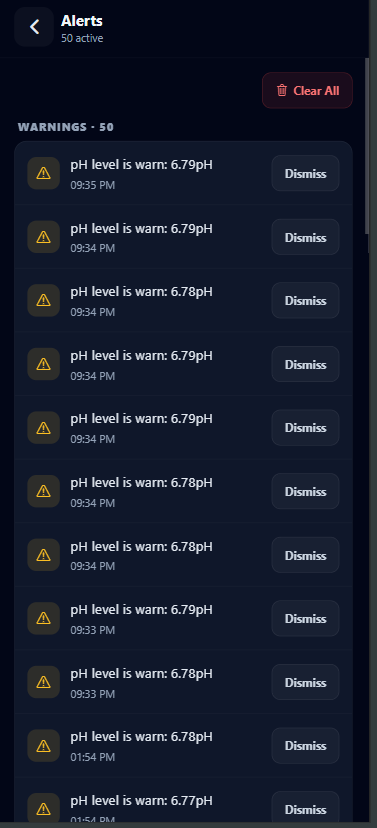
\includegraphics[width=\textwidth]{images/screen_alerts.png}}{\fbox{\parbox[c][4cm][c]{0.9\textwidth}{\centering\itshape [Paste image]\\ \texttt{images/screen\_alerts.png}}}}
        \caption{Alerts screen}
    \end{subfigure}\hfill
    \begin{subfigure}{0.45\textwidth}
        \centering
        \IfFileExists{images/screen_controls.png}{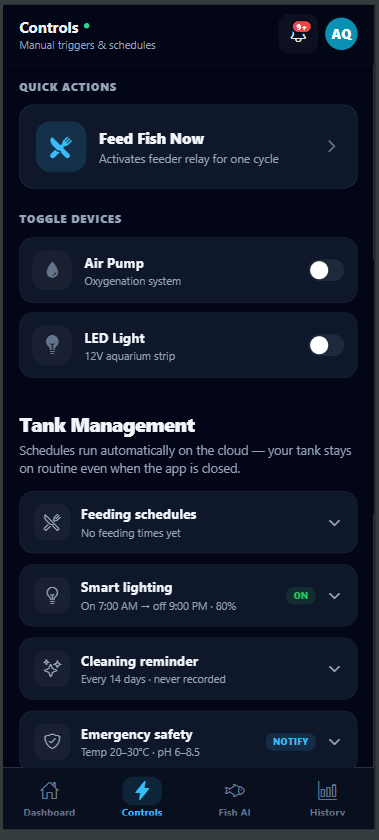
\includegraphics[width=\textwidth]{images/screen_controls.png}}{\fbox{\parbox[c][4cm][c]{0.9\textwidth}{\centering\itshape [Paste image]\\ \texttt{images/screen\_controls.png}}}}
        \caption{Controls screen}
    \end{subfigure}
    \caption{Alerts and Controls screens}
    \label{fig:screens-alerts-controls}
\end{figure}

\subsection{Troubleshooting}
\begin{table}[H]
    \centering\scriptsize
    \begin{tabularx}{\textwidth}{lYl}
        \toprule
        \textbf{Problem} & \textbf{Cause} & \textbf{Solution} \\
        \midrule
        White screen on Expo Go & Metro cache issue & Run \texttt{rm -rf node\_modules/.cache} then restart \\
        Sensors not updating & Arduino disconnected & Check USB connection, verify Serial Monitor \\
        AI predictions failing & FastAPI not running & Run \texttt{cd services/ai-predictor \&\& uvicorn main:app --port 8001} \\
        Veronica not responding & LLM provider unreachable & Verify \texttt{OPENROUTER\_API\_KEY}; app shows \texttt{aiOffline} fallback \\
        Push notifications not received & Invalid push token & Re-register push token in settings \\
        WebSocket disconnects & Network change & App auto-reconnects (max 5 attempts) \\
        Feeder not working & Relay not connected & Check relay wiring (CH1 = feeder) \\
        \bottomrule
    \end{tabularx}
    \caption{Troubleshooting Guide}
\end{table}

\subsection{Maintenance}

\subsubsection{Daily Tasks}
\begin{itemize}
    \item[$\square$] Check sensor readings (verify pH 6.5-8.0, temp 20-30$^\circ$C)
    \item[$\square$] Acknowledge any CRITICAL alerts
    \item[$\square$] Review morning brief (push notification at 07:01)
\end{itemize}

\subsubsection{Weekly Tasks}
\begin{itemize}
    \item[$\square$] Clean pH sensor probe (rinse with distilled water)
    \item[$\square$] Check relay connections (tighten screws if loose)
    \item[$\square$] Review fish growth data (Fish AI screen)
\end{itemize}

\subsubsection{Monthly Tasks}
\begin{itemize}
    \item[$\square$] Calibrate pH sensor (use pH 4.01, 7.01, 10.01 buffer solutions)
    \item[$\square$] Check battery charge level (12V 6000mAh)
    \item[$\square$] Export health reports (Settings $\rightarrow$ Export JSON)
\end{itemize}

% ============================================
% SECTION 7: TESTING & QA
% ============================================
\newpage
\section{Testing \& QA}

\subsection{Test Strategy}
\begin{table}[H]
    \centering\small
    \begin{tabularx}{\textwidth}{YYll}
        \toprule
        \textbf{Test Type} & \textbf{Scope} & \textbf{Tool} & \textbf{Status} \\
        \midrule
        Unit Tests (Backend) & Services, DTOs, Entities & Jest & \textcolor{orange}{Planned} \\
        Integration Tests & API endpoints, WebSocket events & Supertest & \textcolor{orange}{Planned} \\
        E2E Tests (Mobile) & User flows (screens, navigation) & Detox & \textcolor{orange}{Planned} \\
        Hardware Tests & Sensor accuracy, actuator response & Manual & \textcolor{green}{Complete} \\
        AI Model Tests & YOLO mAP, RF accuracy, ConvLSTM AUC & Python (sklearn) & \textcolor{green}{Complete} \\
        \bottomrule
    \end{tabularx}
    \caption{Test Strategy}
\end{table}

\subsection{AI Model Performance}
\begin{table}[H]
    \centering\small
    \begin{tabularx}{\textwidth}{YYll}
        \toprule
        \textbf{Model} & \textbf{Metric} & \textbf{Score} & \textbf{Test Set} \\
        \midrule
        YOLO Disease Detection & mAP@0.5 & 0.87 & 500 images \\
        YOLO Fish Count & MAE & 1.2 fish & 200 images \\
        Random Forest (Water Quality) & R$^2$ & 0.92 & 1000 samples \\
        ConvLSTM-VAE (Behavior) & AUC-ROC & 0.89 & 50 videos \\
        \bottomrule
    \end{tabularx}
    \caption{AI Model Performance}
\end{table}

\figslot{images/model_results.png}{Model evaluation (water-quality comparison + confusion / feature importance)}{fig:model-results}

\subsection{Hardware Test Results}
\begin{table}[H]
    \centering
    \begin{tabularx}{\textwidth}{llll}
        \toprule
        \textbf{Sensor} & \textbf{Expected Range} & \textbf{Measured Range} & \textbf{Accuracy} \\
        \midrule
        pH & 6.5-8.0 & 6.8-7.9 & $\pm$0.15 pH \\
        DO & 4-12 mg/L & 4.2-11.8 mg/L & $\pm$0.4 mg/L \\
        Temp & 20-30$^\circ$C & 20.5-29.8$^\circ$C & $\pm$0.6$^\circ$C \\
        CO$_2$ & 0-10 ppm & 0.02-9.8 ppm & $\pm$0.8 ppm \\
        \bottomrule
    \end{tabularx}
    \caption{Hardware Test Results}
\end{table}

\subsection{Known Issues}
\begin{table}[H]
    \centering\scriptsize
    \begin{tabularx}{\textwidth}{lYll}
        \toprule
        \textbf{Issue} & \textbf{Impact} & \textbf{Workaround} & \textbf{Priority} \\
        \midrule
        Expo Go white screen (macOS) & Mobile app crashes & Clean metro cache, restart & P0 (Fixed) \\
        Local LLM crashes during demos & Veronica unavailable & Migrated to OpenRouter cloud LLM & P1 (Fixed) \\
        \texttt{react-native-reanimated} breaks Expo Go & Animations disabled & Use plain React Native animations & P2 (Won't fix) \\
        Simulated data masks hardware bugs & False confidence & Set \texttt{SIMULATE\_SENSORS=false} & P1 (Fixed) \\
        \bottomrule
    \end{tabularx}
    \caption{Known Issues}
\end{table}

% ============================================
% SECTION 8: API & TECHNICAL SPECIFICATIONS
% ============================================
\newpage
\section{API \& Technical Specifications}

\subsection{REST Endpoints (NestJS :3000)}

\subsubsection{Sensors}
\begin{table}[H]
    \centering
    \begin{tabularx}{\textwidth}{llYY}
        \toprule
        \textbf{Method} & \textbf{Endpoint} & \textbf{Request} & \textbf{Response} \\
        \midrule
        GET & \texttt{/sensors/latest} & -- & \texttt{\{ pH, temp\_c, do\_mg\_l, CO2 \}} \\
        GET & \texttt{/sensors/:id/readings?range=24h} & -- & \texttt{[\{ readingId, value, timestamp \}]} \\
        POST & \texttt{/serial/reading} & \texttt{\{ sensorId, type, value \}} & \texttt{\{ success: boolean \}} \\
        \bottomrule
    \end{tabularx}
    \caption{Sensors Endpoints}
\end{table}

\subsubsection{Actuators}
\begin{table}[H]
    \centering
    \begin{tabularx}{\textwidth}{llYY}
        \toprule
        \textbf{Method} & \textbf{Endpoint} & \textbf{Request} & \textbf{Response} \\
        \midrule
        POST & \texttt{/actuators/feed} & \texttt{\{ cycles: 2 \}} & \texttt{\{ success: boolean \}} \\
        POST & \texttt{/actuators/pump} & \texttt{\{ state: boolean \}} & \texttt{\{ success: boolean \}} \\
        POST & \texttt{/actuators/led} & \texttt{\{ state: boolean \}} & \texttt{\{ success: boolean \}} \\
        POST & \texttt{/actuators/emergency-off} & -- & \texttt{\{ success: boolean \}} \\
        \bottomrule
    \end{tabularx}
    \caption{Actuators Endpoints}
\end{table}

\subsubsection{AI Predictor (Internal)}
\begin{table}[H]
    \centering
    \begin{tabularx}{\textwidth}{llYY}
        \toprule
        \textbf{Method} & \textbf{Endpoint} & \textbf{Request} & \textbf{Response} \\
        \midrule
        POST & \texttt{/predict/quality} & \texttt{\{ pH, temp, do2, co2 \}} & \texttt{\{ score, status \}} \\
        POST & \texttt{/predict/disease} & \texttt{\{ imagePath \}} & \texttt{\{ disease, confidence, bbox \}} \\
        POST & \texttt{/predict/count} & \texttt{\{ imagePath \}} & \texttt{\{ count, confidence \}} \\
        POST & \texttt{/predict/movement} & \texttt{\{ videoPath \}} & \texttt{\{ movementType, anomalyScore \}} \\
        POST & \texttt{/predict/attitude} & \texttt{\{ videoPath \}} & \texttt{\{ tiltSeverity, anomalyScore \}} \\
        \bottomrule
    \end{tabularx}
    \caption{AI Predictor Endpoints}
\end{table}

\subsection{WebSocket Protocol}

\subsubsection{Event Format}
\textbf{Server $\rightarrow$ Client:}
\begin{lstlisting}[language=JSON]
{
  "event": "sensor:update",
  "data": {
    "readingId": 123,
    "sensorId": 1,
    "type": "pH",
    "value": 7.12,
    "unit": "pH",
    "status": "ok",
    "timestamp": "2026-06-06T04:51:00Z"
  }
}
\end{lstlisting}

\textbf{Client $\rightarrow$ Server:}
\begin{lstlisting}[language=JSON]
{
  "event": "command:feed",
  "data": {
    "cycles": 2
  }
}
\end{lstlisting}

\subsubsection{Server $\rightarrow$ Client Events (6 Total)}
\begin{table}[H]
    \centering
    \begin{tabularx}{\textwidth}{lX}
        \toprule
        \textbf{Event} & \textbf{Payload} \\
        \midrule
        \texttt{sensor:update} & \texttt{SensorReading} \\
        \texttt{alert:new} & \texttt{Alert} \\
        \texttt{fish:count} & \texttt{FishCount} \\
        \texttt{health:report} & \texttt{HealthReport} \\
        \texttt{actuator:state} & \texttt{\{ type, state \}} \\
        \texttt{hardware:status} & \texttt{\{ online: boolean \}} \\
        \bottomrule
    \end{tabularx}
    \caption{WebSocket Events (Server to Client)}
\end{table}

\subsection{Hardware Interfaces}

\subsubsection{Serial Protocol (Arduino $\rightarrow$ Serial Bridge)}
\textbf{Baud Rate:} 9600

\textbf{Sensor Reading:}
\begin{lstlisting}[language=JSON]
{
  "sensorId": 1,
  "type": "pH",
  "value": 7.12,
  "unit": "pH",
  "status": "ok"
}
\end{lstlisting}

\textbf{Actuator Command (Serial Bridge $\rightarrow$ Arduino):}
\begin{lstlisting}[language=bash]
CMD:FEED:2
CMD:PUMP:1
CMD:LED:0
CMD:EMERGENCY_OFF
\end{lstlisting}

% ============================================
% SECTION 9: MAINTENANCE & SUPPORT
% ============================================
\newpage
\section{Maintenance \& Support}

\subsection{Monitoring}

\subsubsection{Logs}
\begin{table}[H]
    \centering
    \begin{tabularx}{\textwidth}{lll}
        \toprule
        \textbf{Service} & \textbf{Log Location} & \textbf{Level} \\
        \midrule
        Backend & \texttt{services/backend/logs/} & INFO \\
        Serial Bridge & \texttt{stdout} & DEBUG \\
        AI Predictor & \texttt{stdout} & INFO \\
        Mobile App & Expo DevTools & DEBUG \\
        \bottomrule
    \end{tabularx}
    \caption{Log Locations}
\end{table}

\subsubsection{Health Checks}
\begin{table}[H]
    \centering
    \begin{tabularx}{\textwidth}{ll}
        \toprule
        \textbf{Service} & \textbf{Endpoint} \\
        \midrule
        Backend & \texttt{GET /health} $\rightarrow$ \texttt{\{ status: 'ok' \}} \\
        AI Predictor & \texttt{GET /health} $\rightarrow$ \texttt{\{ status: 'ok' \}} \\
        Serial Bridge & \texttt{GET /health} $\rightarrow$ \texttt{\{ status: 'ok' \}} \\
        Database & (TypeORM) $\rightarrow$ Connection successful \\
        \bottomrule
    \end{tabularx}
    \caption{Health Check Endpoints}
\end{table}

\subsection{Updates}

\subsubsection{Backend Update}
\begin{lstlisting}[language=bash]
cd services/backend
git pull origin develop
pnpm install
pnpm start:dev
\end{lstlisting}

\subsubsection{Mobile App Update}
\begin{lstlisting}[language=bash]
cd apps/mobile
git pull origin develop
pnpm install
expo start --clear
\end{lstlisting}

\subsubsection{AI Model Update}
\begin{lstlisting}[language=bash]
cd services/ai-predictor
git pull origin develop
# Replace model files in models/
uvicorn main:app --port 8001 --reload
\end{lstlisting}

\subsection{Known Issues \& Support}

\subsubsection{FAQ}
\begin{table}[H]
    \centering
    \begin{tabularx}{\textwidth}{lX}
        \toprule
        \textbf{Question} & \textbf{Answer} \\
        \midrule
        Why is the mobile app showing a white screen? & Clean metro cache: \texttt{rm -rf node\_modules/.cache} then restart Expo. \\
        Why are sensors not updating? & Check Arduino USB connection. Verify Serial Monitor shows JSON at 9600 baud. \\
        Why is Veronica not responding? & Check \texttt{OPENROUTER\_API\_KEY} / connectivity. Reflexes still protect the tank; chat shows an offline fallback. \\
        How do I calibrate the pH sensor? & Use pH 4.01, 7.01, 10.01 buffer solutions. See S6.4.3. \\
        How do I export health reports? & Go to Fish AI screen $\rightarrow$ Settings $\rightarrow$ Export JSON. \\
        \bottomrule
    \end{tabularx}
    \caption{FAQ}
\end{table}

\subsubsection{Support Contacts}
\begin{table}[H]
    \centering
    \begin{tabularx}{\textwidth}{llX}
        \toprule
        \textbf{Role} & \textbf{Name} & \textbf{Responsibility} \\
        \midrule
        Lead Architect \& AI Agent & Ismail (ismoiljon1101) & Backend, Mobile, Veronica, DevOps \\
        Hardware & Sarvar & Arduino, Sensors, Actuators \\
        ML Models & Firdavs & YOLO, Random Forest \\
        Database & Maral & Supabase, ConvLSTM-VAE input \\
        \bottomrule
    \end{tabularx}
    \caption{Support Contacts}
\end{table}

% ============================================
% SECTION 10: APPENDICES
% ============================================
\newpage
\section{Appendices}

\subsection{Glossary}
\begin{table}[H]
    \centering
    \begin{tabularx}{\textwidth}{lX}
        \toprule
        \textbf{Term} & \textbf{Definition} \\
        \midrule
        DO & Dissolved Oxygen (mg/L) \\
        pH & Potential of Hydrogen (0-14 scale) \\
        CO$_2$ & Carbon Dioxide (ppm) \\
        YOLO & You Only Look Once (real-time object detection) \\
        ConvLSTM-VAE & Convolutional LSTM Variational Autoencoder (behavior analysis) \\
        mAP & mean Average Precision (object detection metric) \\
        MAE & Mean Absolute Error (regression metric) \\
        AUC-ROC & Area Under ROC Curve (classification metric) \\
        Expo Go & Expo's sandbox app for running React Native apps without building \\
        Socket.IO & Real-time bidirectional event-based communication (WebSocket) \\
        TypeORM & TypeScript ORM (Object-Relational Mapping) \\
        NestJS & Progressive Node.js framework (inspired by Angular) \\
        FastAPI & Modern Python web framework (based on Starlette + Pydantic) \\
        \bottomrule
    \end{tabularx}
    \caption{Glossary}
\end{table}

\subsection{Image Insertion Guide}
Every figure in this document uses a \texttt{\textbackslash figslot} that shows a labelled
placeholder until the named file exists --- so the PDF \emph{always compiles}. To fill a figure,
drop a file with the exact name below. Diagram renders go in \texttt{docs/}; screenshots and
photos go in \texttt{docs/team/images/} (create that folder).

\begin{table}[H]
    \centering\small
    \begin{tabularx}{\textwidth}{llX}
        \toprule
        \textbf{Expected file} & \textbf{Figure} & \textbf{How to obtain} \\
        \midrule
        \texttt{docs/architecture.png} & High-level architecture & Diagram render or drawn figure \\
        \texttt{docs/ER\_MODEL.png} & ER model & \texttt{mmdc -i docs/ER\_MODEL.mmd -o docs/ER\_MODEL.png} \\
        \texttt{docs/WF\_DIAGRAM.png} & Workflow diagram & \texttt{mmdc -i docs/WF\_DIAGRAM.mmd -o docs/WF\_DIAGRAM.png} \\
        \texttt{images/veronica\_chat.png} & Veronica chat & Mobile screenshot (Fish AI tab) \\
        \texttt{images/veronica\_confirm.png} & Confirm-before-act card & Mobile screenshot \\
        \texttt{images/veronica\_terminal.png} & Reasoning terminal & Mobile screenshot \\
        \texttt{images/screen\_dashboard.png} & Dashboard screen & Mobile screenshot \\
        \texttt{images/screen\_alerts.png} & Alerts screen & Mobile screenshot \\
        \texttt{images/screen\_controls.png} & Controls screen & Mobile screenshot \\
        \texttt{images/hardware\_build.png} & Hardware build & Photo of Arduino + sensors \\
        \texttt{images/model\_results.png} & Model evaluation & \texttt{docs/Water quality/results/*.png} \\
        \bottomrule
    \end{tabularx}
    \caption{Image Insertion Guide}
\end{table}

\textit{Note:} the \texttt{images/} paths are relative to \texttt{docs/team/} (where this
\texttt{.tex} lives); \texttt{docs/} renders are reached via the configured \texttt{graphicspath}.

\subsection{Mobile App Screenshots}
The following screenshots show the mobile app in action. Portrait mobile screenshots are
shown at 35\% text width (preserving readability) with descriptive text beside them.

% --- Veronica Chat ---
\begin{figure}[H]
  \centering
  \begin{minipage}[t]{0.35\textwidth}
    \centering
    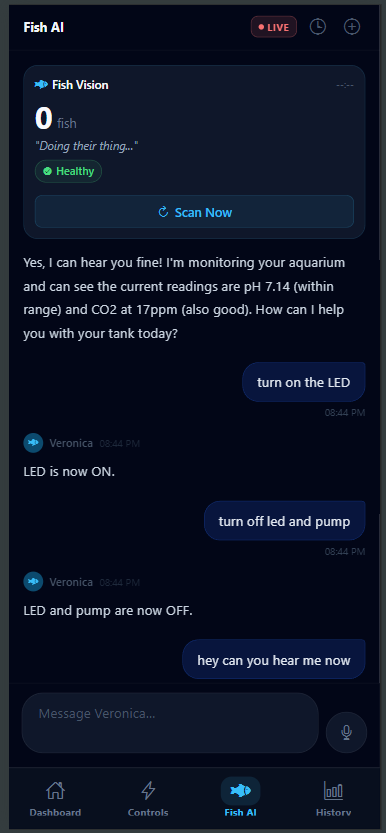
\includegraphics[width=\linewidth]{images/veronica_chat.png}
  \end{minipage}
  \hfill
  \begin{minipage}[t]{0.60\textwidth}
    \raggedright
    \textbf{Veronica Chat Screen} \\
    Users chat with Veronica AI assistant. Type a message, and Veronica analyzes live sensor data,
    checks tank conditions, and can trigger actions (feed, LED, pump) with confirm-before-act.
  \end{minipage}
  \caption{Veronica AI Chat Interface}
  \label{fig:app-veronica-chat}
\end{figure}

% --- Veronica Confirm ---
\begin{figure}[H]
  \centering
  \begin{minipage}[t]{0.35\textwidth}
    \centering
    \includegraphics[width=\linewidth]{images/veronica_confirm.png}
  \end{minipage}
  \hfill
  \begin{minipage}[t]{0.60\textwidth}
    \raggedright
    \textbf{Confirm-Before-Act Card} \\
    When Veronica decides to take an action, she shows a card with the proposed action and reasoning.
    The user must confirm before any actuator changes the tank environment. \\
    \textit{Note: this card only appears when ``Confirm before act'' is enabled in Settings.
    In Auto mode, Veronica executes actions immediately without asking.}
  \end{minipage}
  \caption{Veronica Confirm-Before-Act UI (Settings toggle)}
  \label{fig:app-veronica-confirm}
\end{figure}

% --- Dashboard ---
\begin{figure}[H]
  \centering
  \begin{minipage}[t]{0.35\textwidth}
    \centering
    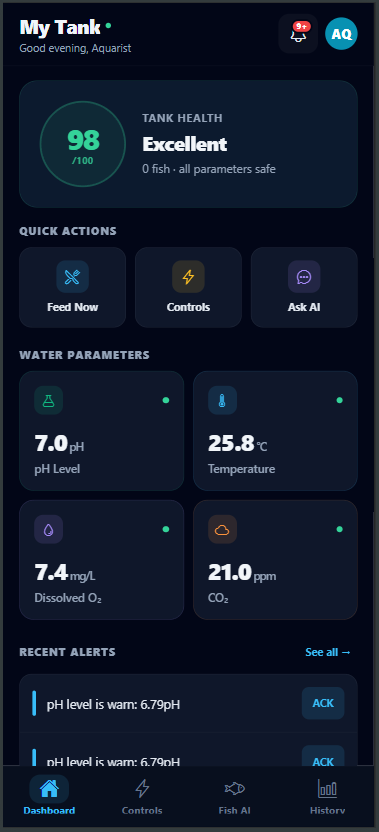
\includegraphics[width=\linewidth]{images/screen_dashboard.png}
  \end{minipage}
  \hfill
  \begin{minipage}[t]{0.60\textwidth}
    \raggedright
    \textbf{Dashboard Screen} \\
    Live sensor cards show pH, temperature, DO2, CO2 with color-coded status badges.
    The health score hero gives an at-a-glance view of tank condition.
  \end{minipage}
  \caption{Mobile Dashboard — Live Sensor Data}
  \label{fig:app-dashboard}
\end{figure}

% --- Alerts ---
\begin{figure}[H]
  \centering
  \begin{minipage}[t]{0.35\textwidth}
    \centering
    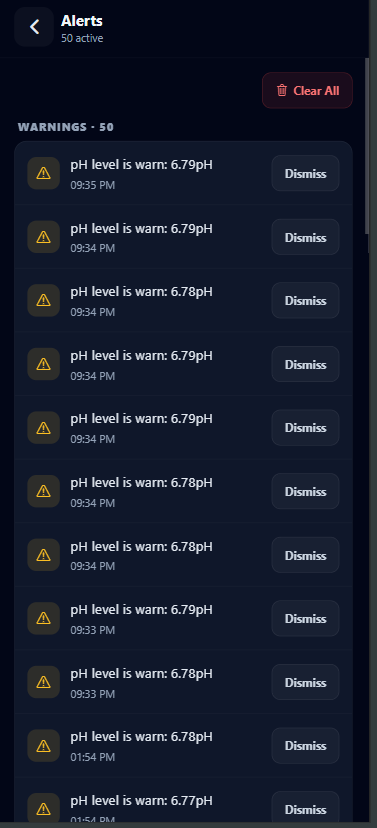
\includegraphics[width=\linewidth]{images/screen_alerts.png}
  \end{minipage}
  \hfill
  \begin{minipage}[t]{0.60\textwidth}
    \raggedright
    \textbf{Alerts Screen} \\
    Active alerts listed with severity (INFO / WARNING / CRITICAL / EMERGENCY).
    Swipe to acknowledge. Alert count badge on tab icon.
  \end{minipage}
  \caption{Mobile Alerts Screen}
  \label{fig:app-alerts}
\end{figure}

% --- Controls ---
\begin{figure}[H]
  \centering
  \begin{minipage}[t]{0.35\textwidth}
    \centering
    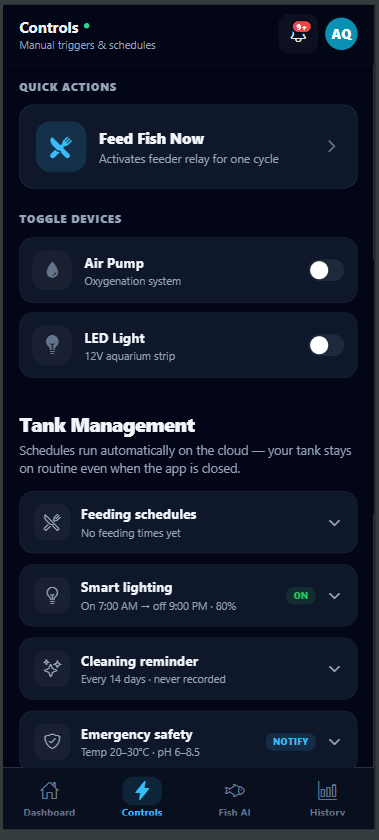
\includegraphics[width=\linewidth]{images/screen_controls.png}
  \end{minipage}
  \hfill
  \begin{minipage}[t]{0.60\textwidth}
    \raggedright
    \textbf{Controls Screen} \\
    Manual override for Feeder, Air Pump, and LED Strip. Emergency Stop button disables all actuators.
    Tank config and light/feed schedules managed here.
  \end{minipage}
  \caption{Mobile Controls — Actuator Override}
  \label{fig:app-controls}
\end{figure}

\subsection{References}
\begin{table}[H]
    \centering
    \begin{tabularx}{\textwidth}{lX}
        \toprule
        \textbf{Reference} & \textbf{Link} \\
        \midrule
        Repository & \url{https://github.com/ismoiljon1101/capstone_aquarium_sejong} \\
        NestJS Documentation & \url{https://docs.nestjs.com} \\
        Expo Documentation & \url{https://docs.expo.dev} \\
        FastAPI Documentation & \url{https://fastapi.tiangolo.com} \\
        TypeORM Documentation & \url{https://typeorm.io} \\
        Socket.IO Documentation & \url{https://socket.io/docs} \\
        YOLOv8 Documentation & \url{https://docs.ultralytics.com} \\
        ConvLSTM-VAE Paper & \url{https://arxiv.org/abs/2003.06565} \\
        Supabase Documentation & \url{https://supabase.com/docs} \\
        \bottomrule
    \end{tabularx}
    \caption{References}
\end{table}

\subsection{Changelog}
\begin{table}[H]
    \centering\small
    \begin{tabularx}{\textwidth}{llX}
        \toprule
        \textbf{Version} & \textbf{Date} & \textbf{Changes} \\
        \midrule
        v1.0 & 2026-05-15 & Initial documentation (basic structure) \\
        v1.5 & 2026-06-05 & Added ER models, expanded API specs \\
        v2.0 & 2026-06-06 & Complete IEEE-inspired restructure, added ER diagrams, expanded all sections \\
        v3.0 & 2026-06-06 & Corrected ownership (129/152), rewrote Veronica with the real 17-tool agent + deterministic safety layer, real cron jobs, image slots, brand fix (Fishlinic) \\
        \bottomrule
    \end{tabularx}
    \caption{Changelog}
\end{table}

% ============================================
% DOCUMENT APPROVAL
% ============================================
\newpage
\section*{Document Approval}

\begin{table}[H]
    \centering\small
    \begin{tabularx}{\textwidth}{lYll}
        \toprule
        \textbf{Role} & \textbf{Name} & \textbf{Signature} & \textbf{Date} \\
        \midrule
        Lead Architect & Ismoiljon (ismoiljon1101) & $\square$ & 2026-06-06 \\
        Team Member & Maral & $\square$ & -- \\
        Team Member & Sarvar & $\square$ & -- \\
        Team Member & Firdavs & $\square$ & -- \\
        Institution & Sejong University & $\square$ & -- \\
        \bottomrule
    \end{tabularx}
\end{table}

\vfill
\begin{center}
    \textit{This document is the complete technical documentation for the Fishlinic smart aquarium monitoring system.}\\
    \textit{For questions or clarifications, contact the Lead Architect (ismoiljon1101@gmail.com).}
\end{center}

\end{document}
